\subsection{Training labels and the grouped data division}
\label{sec:seed-model-split}
For each target, let $\mathcal S_{\mathcal T}\subseteq\mathcal C$
be the sufficient seed set used by its recorded reduction.
The reference label for candidate $b$ is
\begin{equation}
 y_b(\mathcal T)=
 \begin{cases}
 1,&\boldsymbol\sigma_b\in\mathcal S_{\mathcal T},\\
 0,&\boldsymbol\sigma_b\notin\mathcal S_{\mathcal T}.
 \end{cases}
 \label{eq:seed-membership-label}
\end{equation}
A zero label records absence from this particular set; another valid
reduction can use that seed. Algebraic mass partial fractions carry
no seed label. For example, a target whose reference uses the first
and third of five candidates has
\begin{equation}
 \boldsymbol y(\mathcal T)=(1,0,1,0,0).
 \label{eq:seed-label-example}
\end{equation}
The target coefficients and public family information enter the
prediction, while this label vector enters the training loss.

We keep each family together and preserve the grouping of related
mass and kinematic profiles described in
Section~\ref{sec:higher-loop-generation}. The expanded division
contains @TRAIN_TARGETS@ training targets in @TRAIN_FAMILIES@
families and @TEST_TARGETS@ test targets in @TEST_FAMILIES@
families. Every loop order from one through twelve occurs in both
sets. Each added mass profile stays in one set across all loop orders.
The ratio applies to complete target examples, each with its full
candidate list. Shared lower-sector integrals can occur across
different profiles, and the original held-out families were also
evaluated in earlier project stages.

The training objective gives each target equal weight:
\begin{equation}
 \mathcal L(\theta)=
 -\frac{1}{|\mathcal D_{\rm train}|}
 \sum_{\mathcal T\in\mathcal D_{\rm train}}
 \frac{1}{n_C(\mathcal T)}
 \sum_{b=1}^{n_C(\mathcal T)}
 \left[y_b\log p_b+(1-y_b)\log(1-p_b)\right].
 \label{eq:seed-training-loss}
\end{equation}
Here $\mathcal D_{\rm train}$ is the training set and
$n_C(\mathcal T)$ is the candidate count for target $\mathcal T$.
All positive and zero labels enter this binary cross-entropy without
additional class weighting. The threshold of one half determines
reported decisions after the model supplies its probabilities.

\subsection{Completed training and implementation checks}
We continued the saved model and its AdamW optimizer on the expanded
training set for twenty complete passes. The starting checkpoint
had completed @PRIOR_EPOCHS@ passes over the earlier collection and
@PRIOR_PARTIAL@ targets in its next pass. The new phase retains this
learned state and uses its own twenty-pass counter. It contains
@PRESENTATIONS@ target presentations and @UPDATES@ parameter updates.

The architecture still has 28,097 parameters. AdamW uses a learning
rate of $10^{-3}$, weight decay of $10^{-4}$ and a maximum gradient
norm of one~\cite{AdamW}. Each update uses up to 32 targets from a
training family. We change family and target order between passes
and use the actual batch size for the final group. Masked batch
calculations retain every target term, every ordered pair of
distinct terms and every supplied seed. Comparisons with the
individual-target calculation verified matching scores, losses and
parameter derivatives across individual-integral and multi-term examples.

The mean training loss changed from @FIRST_LOSS@ in the first
expanded-data pass to @LAST_LOSS@ in the twentieth.
Figure~\ref{fig:training-loss} shows the complete history.
These means include parameter changes within each pass and describe
fitting on the training examples.

\begin{figure}[htbp]
 \centering
 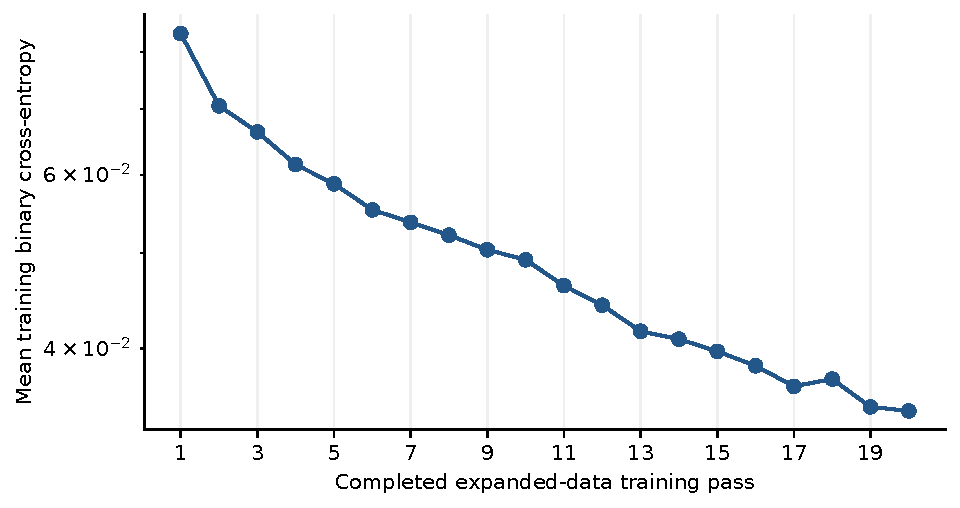
\includegraphics[width=0.80\linewidth]{figures/training_loss.pdf}
 \caption{Mean training binary cross-entropy during the twenty
 expanded-data passes. Each target has equal weight within the
 reported mean. The logarithmic vertical axis shows the training
 history; held-out examples do not enter this curve.}
 \label{fig:training-loss}
\end{figure}

The checks verify target-label correspondence, membership of every
recorded seed in the candidate pool, complete coverage during each
pass, and equality of the published weights with the resumable
checkpoint. The model retains the separate class probabilities and
confidence rule in Eq.~\eqref{eq:seed-binary-confidence}.
Held-out examples supplied no gradient updates or threshold fitting.

The representation accepts up to sixteen indices, 512 target terms
and 10,000 supplied candidates. The added twelve-loop examples reach
the index limit. This capacity describes the input representation;
the training evidence concerns the actual family domains defined
above. Section~\ref{sec:seed-test-results} evaluates the frozen
parameters on their reserved mass profiles.
\FloatBarrier
